% ============================================================================
%  PROPOSAL BODY — counted against the 10-page limit.
% ============================================================================

% ----------------------------------------------------------------------------
\section{Executive Summary \& Value Proposition}
% ----------------------------------------------------------------------------

Every year, millions of Indonesian students are judged against a written rubric
they have already been given: a hackathon scoring matrix, a scholarship
interview guide, a thesis examination form. The rubric is rarely secret. What
students lack is not the criteria but a way to \emph{practise against them} and
find out, before the room, which of their claims will not survive a question.

The support that closes that gap is a mentor who reads your rubric, listens,
and asks the hard question. It is also the scarcest resource in Indonesian
higher education, and it is distributed by luck: by faculty, by alumni network,
by whether a senior has time. Students without that access do not practise less;
they practise blindly, rehearsing fluency while their weakest claim stays
invisible until an evaluator names it.

\ProductName{} is an AI rehearsal workspace that makes the evaluator's own
rubric the centre of practice. A student enters the real scoring criteria and
rehearses. \ProductName{} maps every claim in the transcript to a criterion,
shows which are supported and which are merely asserted, identifies the weakest
defensible claim, and generates the question a skeptical evaluator would ask
about it. The student answers, learns which evidence landed, and saves the
session. Across attempts, the workspace surfaces the weakness that keeps
recurring.

\callout{\textbf{Value proposition.} Existing AI speaking tools coach
\emph{delivery}: pace, filler words, confidence. They are rubric-blind: they
cannot tell a student that a market-size claim is unsupported, because they do
not know the student is being scored on market size. \ProductName{} inverts the
input. The rubric comes first, and every piece of feedback cites a criterion and
the exact sentence that did or did not satisfy it. This is not a better speaking coach.
It is the rehearsal layer for \emph{evaluation itself}.}

The differentiating loop is \textbf{project → rubric →
attempt → traceable evidence → hardest question
→ saved progress}. The loop is narrow and repeatable, which makes it
testable with real students instead of merely impressive in a demo.

\textbf{Current status.} A working prototype already runs as a deployed web
application, covering projects, rubric editing, evidence review, question
generation, and saved history, verified by an automated gate of 15 unit tests
and 11 browser checks. We also used it on ourselves: \textbf{we entered this
guidebook's own scoring matrix as a rubric and ran our pitch through it}, and it
named Business Strategy as our weakest criterion, so we rewrote the pitch to
lead with market sizing and revenue. Its analysis today is deterministic cue
matching, not semantic understanding, a boundary Section~4.4 states plainly and
the Innovation Week sprint is scoped to replace.

% ----------------------------------------------------------------------------
\section{Problem Identification}
% ----------------------------------------------------------------------------

\subsection{The problem and its scale}

Indonesia's higher education system enrolled \textbf{9,949,502 students} as of
December 2025, of whom \textbf{8,281,591} are undergraduates
\cite{pddikti2025}. Nearly all will face at least one rubric-scored oral
evaluation before graduating: a thesis defense, a job interview, a scholarship
panel, a competition pitch. Each one is high-stakes, single-shot, and scored
against criteria the student can usually read in advance. Two pressures make this
pressing rather than routine.

\textbf{First, the anxiety is near-universal and documented.} A study of
first-year Indonesian university students found \textbf{63\% at moderate and
18\% at high levels} of public speaking anxiety, so 81\% of the cohort was
affected
\cite{educasia2024}; a separate study of fifth-semester students reported
\textbf{53.33\% at high levels} \cite{leea2023}. At this prevalence it is not a
personality trait to be coached away, but a predictable response to being
evaluated without ever having rehearsed under evaluative conditions.

\textbf{Second, the selection funnels are narrow and getting narrower.} LPDP, the
country's flagship government scholarship, grew from roughly 25,000 applicants
in 2022 to approximately 78,000 in 2025. In Stage~2 of the 2025 cycle,
\textbf{37,459 applicants} competed and only \textbf{2,511} passed the
substance selection, an interview-stage pass rate near \textbf{6.7\%}
\cite{lpdp2025,goodstats2025}. At that ratio the interview is not a formality
confirming a strong file; it is the decisive filter, and the stage students can
least afford to practise alone.

% ---------------------------------------------------------------- Figure ----
% Problem evidence: the selection funnel and the anxiety base rate.
\begin{figure}[htbp]
\centering
\begin{tikzpicture}[font=\fontsize{8}{9.5}\selectfont]

% ============================ PANEL A : LPDP selection funnel ==============
\begin{scope}[xshift=0cm]

  \node[font=\fontsize{9}{11}\selectfont\bfseries, text=inkgrey, anchor=west]
    at (0,3.25) {(a) LPDP 2025 Stage 2: the interview is the filter};

  % funnel bars (width proportional to volume, log-ish for legibility)
  \fill[uinavy!75, rounded corners=1.5pt] (0,2.35) rectangle (6.6,2.85);
  \node[anchor=west, text=white, font=\fontsize{8}{9}\selectfont\bfseries]
    at (0.12,2.60) {37,459 applicants entered Stage 2};

  \fill[uinavy!45, rounded corners=1.5pt] (0,1.70) rectangle (4.3,2.20);
  \node[anchor=west, text=white, font=\fontsize{8}{9}\selectfont\bfseries]
    at (0.12,1.95) {administrative + scholastic screening};

  \fill[uired!85, rounded corners=1.5pt] (0,1.05) rectangle (0.44,1.55);
  \node[anchor=west, text=uired, font=\fontsize{8}{9}\selectfont\bfseries]
    at (0.56,1.30) {2,511 passed substance selection};

  % the ratio callout
  \node[draw=uired!55, fill=uired!7, line width=0.5pt, rounded corners=2pt,
        inner sep=4pt, text width=6.3cm, align=left,
        font=\fontsize{8}{9.5}\selectfont, anchor=north west] at (0,0.80)
    {\textbf{\textcolor{uired}{≈6.7\% pass the interview stage.}}
     One attempt, no feedback, no rehearsal partner. Applicant volume grew from
     about 25,000 (2022) to about 78,000 (2025).};

\end{scope}

% ============================ PANEL B : anxiety base rate ==================
\begin{scope}[xshift=7.9cm]

  \node[font=\fontsize{9}{11}\selectfont\bfseries, text=inkgrey, anchor=west]
    at (0,3.25) {(b) Public speaking anxiety, first-year students};

  % stacked horizontal bar, total width 6.4cm = 100%
  \def\W{6.4}
  \fill[uired!80,   rounded corners=1.5pt] (0,2.30) rectangle ({\W*0.18},2.85);
  \fill[warnamber!70]                      ({\W*0.18},2.30) rectangle ({\W*0.81},2.85);
  \fill[goodgreen!55, rounded corners=1.5pt] ({\W*0.81},2.30) rectangle ({\W},2.85);

  \node[text=white, font=\fontsize{7.6}{9}\selectfont\bfseries] at ({\W*0.09},2.575) {18\%};
  \node[text=white, font=\fontsize{7.6}{9}\selectfont\bfseries] at ({\W*0.50},2.575) {63\%};
  \node[text=white, font=\fontsize{7.6}{9}\selectfont\bfseries] at ({\W*0.905},2.575) {19\%};

  % legend
  \fill[uired!80] (0,1.90) rectangle (0.22,2.06);
  \node[anchor=west, font=\fontsize{7.8}{9}\selectfont] at (0.28,1.98) {High anxiety};
  \fill[warnamber!70] (2.25,1.90) rectangle (2.47,2.06);
  \node[anchor=west, font=\fontsize{7.8}{9}\selectfont] at (2.53,1.98) {Moderate};
  \fill[goodgreen!55] (4.55,1.90) rectangle (4.77,2.06);
  \node[anchor=west, font=\fontsize{7.8}{9}\selectfont] at (4.83,1.98) {Low};

  \node[draw=warnamber!55, fill=warnamber!7, line width=0.5pt, rounded corners=2pt,
        inner sep=4pt, text width=6.3cm, align=left,
        font=\fontsize{8}{9.5}\selectfont, anchor=north west] at (0,1.62)
    {\textbf{\textcolor{warnamber}{81\% report moderate or high anxiety.}}
     A separate cohort study of fifth-semester students found 53.3\% at high
     levels. This is a predictable response to being evaluated without ever
     having rehearsed under evaluative conditions.};

\end{scope}

\end{tikzpicture}
\caption{The problem is measurable on two axes: the selection funnel is
punishing, and the anxiety it produces is close to universal.
Sources: \cite{lpdp2025,goodstats2025,educasia2024,leea2023}.}
\label{fig:problem}
\end{figure}


\callout{The gap is not information and not effort. Students can obtain the
rubric and they do rehearse. What they cannot obtain is an evaluator who will
read that rubric, listen, and tell them which specific claim is weakest, then
ask about it. \textbf{Rehearsal quality is currently a function of network
access, and that is an equity problem.}}

\subsection{Target users and their pain points}

Our initial user is an Indonesian undergraduate facing a rubric-driven oral
evaluation within the next four to eight weeks, with limited or no mentor
access. Table~\ref{tab:persona} defines the three segments we design for, in
priority order.

\begin{table}[htbp]
\centering
\caption{Target personas and the specific pain point each one brings.}
\label{tab:persona}
{\fontsize{10.5}{13}\selectfont
\begin{tabularx}{\textwidth}{@{}L{2.6cm} L{3.5cm} X@{}}
\toprule
\textbf{Persona} & \textbf{Context} & \textbf{Specific pain point} \\
\midrule
\textbf{The competitor}\newline (beachhead) &
Undergraduate in a hackathon, business case, or scientific paper competition.
Rubric is published with the guidebook. &
Knows the scoring matrix but cannot tell which criterion the pitch currently
under-serves. Discovers the gap during Q\&A, when it is too late to fix. \\
\addlinespace
\textbf{The defender} &
Final-year student preparing a thesis or internship defense against a
standard examination form. &
Rehearses the presentation but never the interrogation. Cannot predict which
claim the examiner will attack, and has no one to play examiner. \\
\addlinespace
\textbf{The applicant} &
Scholarship (LPDP, Chevening, Australia Awards) or first-job candidate. &
Faces an interview funnel near 6.7\% with one attempt. Practises answers in
isolation with no feedback on whether an answer is actually defensible. \\
\bottomrule
\end{tabularx}}
\end{table}

Across all three, the same four failures recur: the student cannot locate the
weakest claim; cannot anticipate the follow-up question; receives feedback on
delivery rather than substance; and has no record of whether the same weakness
keeps returning across attempts.

\subsection{Alignment with the grand theme}

The theme asks for technology that looks past commercial metrics to a societal
problem. Preparation inequality is exactly that: two students of equal ability
do not get equal outcomes when only one has access to someone who will rehearse
them properly. \ProductName{} takes the rubric, the one input that is already
public and equally available, and turns it into the rigorous, repeated,
question-driven practice currently reserved for the well-connected. This sits
within the \textbf{\SubTheme{}} sub-theme's call for digital upskilling and
equitable access, and advances the Indonesia Emas 2045 objective of a
competitive, future-ready generation.

% ----------------------------------------------------------------------------
\section{Solution Overview \& Innovation}
% ----------------------------------------------------------------------------

\subsection{The rubric-grounded rehearsal loop}

\ProductName{} treats the rubric as the primary object in the system, not as
decoration. Figure~\ref{fig:loop} shows the loop a student repeats.

% ---------------------------------------------------------------- Figure 1 --
% The core rehearsal loop.
\begin{figure}[htbp]
\centering
\begin{tikzpicture}[
  font=\fontsize{8.5}{10}\selectfont,
  stage/.style={
    draw=ristekpurple!55, fill=softpurple, line width=0.6pt,
    rounded corners=2.5pt, minimum height=1.15cm, text width=1.72cm,
    align=center, inner sep=3pt
  },
  flow/.style={-{Stealth[length=4pt]}, draw=ristekpurple!75, line width=0.7pt}
]

\node[stage] (p1) {\textbf{1. Project}\\[1pt] real event\\ \& deadline};
\node[stage, right=0.30cm of p1] (p2) {\textbf{2. Rubric}\\[1pt] evaluator's\\ real criteria};
\node[stage, right=0.30cm of p2] (p3) {\textbf{3. Attempt}\\[1pt] speak or\\ paste draft};
\node[stage, right=0.30cm of p3] (p4) {\textbf{4. Evidence}\\[1pt] cited per\\ criterion};
\node[stage, right=0.30cm of p4] (p5) {\textbf{5. Question}\\[1pt] on weakest\\ claim};
\node[stage, right=0.30cm of p5] (p6) {\textbf{6. Save}\\[1pt] progress \&\\ recurring gap};

\foreach \a/\b in {p1/p2, p2/p3, p3/p4, p4/p5, p5/p6}{\draw[flow] (\a) -- (\b);}

% return arrow: the loop closes back onto the next attempt
\draw[flow, dashed]
  (p6.south) -- ++(0,-0.42)
  -| node[pos=0.25, below, font=\fontsize{8}{9}\selectfont\itshape, text=ristekpurple!90]
     {the next attempt starts from what the last one exposed} (p3.south);

\end{tikzpicture}
\caption{The rubric-grounded rehearsal loop. Each stage feeds the next, and the
saved session conditions the following attempt.}
\label{fig:loop}
\end{figure}


Each stage produces something the next stage consumes, and the loop closes: the
saved session is what makes the next attempt smarter than the last. Two
properties matter more than the individual steps. Preparation is organised
around one real event rather than generic exercises, so the rubric stays
attached to the thing being prepared for. And no verdict reaches the student
without a citation, so every critique can be traced back to a criterion the
evaluator wrote and a sentence the student actually said.

\subsection{Differentiation}

The AI speaking-coach category is real and funded, so differentiation must be
stated precisely rather than claimed. Table~\ref{tab:diff} compares
\ProductName{} against the established tools.

\begin{table}[htbp]
\centering
\caption{Differentiation against existing market alternatives.}
\label{tab:diff}
{\fontsize{9.5}{11.2}\selectfont
\begin{tabularx}{\textwidth}{@{}L{3.15cm} C{1.85cm} C{1.6cm} C{1.5cm} X@{}}
\toprule
\textbf{Capability} & \textbf{Yoodli} & \textbf{Orai} & \textbf{Poised} &
\textbf{\ProductName{}} \\
\midrule
Primary input & Speech & Speech & Live call &
\textbf{The evaluator's rubric} \\
Feedback target & Delivery & Delivery & Delivery &
\textbf{Substance per criterion} \\
Claims cited to a criterion & No & No & No & \textbf{Always} \\
Generates the judge's next question & Generic roleplay & No & No &
\textbf{From the weakest claim} \\
Tracks recurring substantive gaps & Session stats & Streaks & No &
\textbf{Per-criterion, across attempts} \\
Indonesian evaluation context & Limited & Limited & No &
\textbf{Native (ID/EN)} \\
Indicative price & USD 8--20/mo & USD 10/mo & Subscription &
\textbf{Free; Rp39k/mo Pro} \\
\bottomrule
\end{tabularx}}
\end{table}

% ---------------------------------------------------------------- Figure ----
% Competitive positioning: what the category optimises for vs. what we do.
\begin{figure}[htbp]
\centering
\begin{tikzpicture}[font=\fontsize{8}{9.5}\selectfont]

\def\W{11.6}   % plot width
\def\H{4.9}    % plot height
\pgfmathsetmacro{\Mx}{\W/2}
\pgfmathsetmacro{\My}{\H/2}

% quadrant background
\fill[panelgrey, rounded corners=3pt] (0,0) rectangle (\W,\H);
\fill[softpurple] ({\Mx},{\My}) rectangle ({\W-0.02},{\H-0.02});

% grid + frame
\draw[rulegrey, line width=0.6pt] ({\Mx},0) -- ({\Mx},\H);
\draw[rulegrey, line width=0.6pt] (0,{\My}) -- (\W,{\My});
\draw[rulegrey, line width=0.7pt, rounded corners=3pt] (0,0) rectangle (\W,\H);

% ---- axis labels ----------------------------------------------------------
\node[font=\fontsize{8.4}{10}\selectfont, text=inkgrey]
  at ({\Mx},-0.40)
  {grounded in generic speech → \textbf{in the evaluator's actual rubric}};
\node[font=\fontsize{8.4}{10}\selectfont, text=inkgrey, rotate=90]
  at (-0.42,{\My})
  {targets delivery → \textbf{substance}};

% ---- quadrant captions ----------------------------------------------------
\node[font=\fontsize{7.6}{9}\selectfont\itshape, text=inkgrey!65, anchor=north west]
  at (0.14,{\H-0.10}) {substance, but rubric-blind};
\node[font=\fontsize{7.6}{9}\selectfont\itshape, text=inkgrey!65, anchor=south west]
  at (0.14,0.12) {delivery coaching};
\node[font=\fontsize{7.6}{9}\selectfont\itshape, text=inkgrey!65, anchor=south east]
  at ({\W-0.14},0.12) {rubric-aware, but still delivery};
\node[font=\fontsize{7.8}{9.4}\selectfont\bfseries, text=ristekpurple, anchor=north east]
  at ({\W-0.14},{\H-0.10}) {rubric-grounded rehearsal};

% ---- plotted players ------------------------------------------------------
% #1 x  #2 y  #3 name  #4 sublabel
\newcommand{\player}[4]{%
  \node[circle, draw=inkgrey!60, fill=white, line width=0.6pt,
        minimum size=0.26cm, inner sep=0pt] at (#1,#2) {};
  \node[anchor=west, align=left, font=\fontsize{8}{9.4}\selectfont, text=inkgrey]
    at ({#1+0.20},#2)
    {\textbf{#3}~{\fontsize{6.9}{8}\selectfont\itshape\color{inkgrey!75}#4}};
}

\player{1.05}{0.72}{Orai}{delivery, streaks}
\player{1.05}{1.62}{Poised}{live-call cues}
\player{3.95}{1.17}{Yoodli}{+ generic roleplay}
\player{1.30}{3.60}{Human mentor}{ideal, but scarce}

% Talk-Active, emphasised
\node[circle, draw=ristekpurple, fill=ristekpurple, line width=0.8pt,
      minimum size=0.40cm, inner sep=0pt] at (7.05,3.60) {};
\node[anchor=west, align=left, text=ristekpurple] at (7.30,3.60)
  {\fontsize{10.5}{12}\selectfont\bfseries \ProductName{}\\[-1.5pt]
   {\fontsize{7}{8.2}\selectfont\itshape every verdict cites a criterion}};

\end{tikzpicture}
\caption{Competitive positioning. The category optimises delivery, leaving the
quadrant that decides evaluation outcomes unoccupied. A delivery coach cannot
enter it by adding a feature: the rubric has to be the primary key of the data
model, not one more input to a prompt.}
\label{fig:compete}
\end{figure}


\callout{\textbf{The unique logic, stated plainly.} A generic coach can tell a
student they said ``um'' eleven times. Only a rubric-grounded system can tell
them that \emph{Criterion 3 asks for field data and the pitch offered an
anecdote}, then ask the question the judge was going to ask. This is not a
model choice or a prompt; it is an architecture in which the rubric, not the
audio, is the primary key. That is why it is hard to clone by adding a feature
to a delivery coach.}

% ----------------------------------------------------------------------------
\section{Technical Architecture \& Tech Stack}
% ----------------------------------------------------------------------------

\subsection{System architecture}

\ProductName{} is a web application built on a serverless platform, chosen so
that a five-person student team can operate it reliably without managing
infrastructure. Figure~\ref{fig:arch} shows the target architecture for the
Innovation Week build.

% ---------------------------------------------------------------- Figure 2 --
% Target system architecture and data flow.
\begin{figure}[htbp]
\centering
\begin{tikzpicture}[
  font=\fontsize{8.2}{9.6}\selectfont,
  svc/.style={
    draw=ristekpurple!55, fill=white, line width=0.55pt, rounded corners=2pt,
    minimum height=0.82cm, text width=2.62cm, align=center, inner sep=2.5pt
  },
  ai/.style={svc, draw=uired!55, fill=uired!6},
  store/.style={svc, draw=uinavy!55, fill=uinavy!6},
  band/.style={
    draw=rulegrey, fill=panelgrey, line width=0.5pt, rounded corners=3pt
  },
  lbl/.style={font=\fontsize{8}{9}\selectfont\bfseries, text=inkgrey},
  flow/.style={-{Stealth[length=3.6pt]}, draw=inkgrey!70, line width=0.6pt}
]

% ---------------- Layer 1: client
\node[svc, fill=softpurple, draw=ristekpurple!70] (web)
  {\textbf{Next.js Web App}\\ React, TypeScript};
\node[svc, fill=softpurple, draw=ristekpurple!70, right=0.5cm of web] (rec)
  {\textbf{Recorder}\\ browser audio capture};
\node[svc, fill=softpurple, draw=ristekpurple!70, right=0.5cm of rec] (auth)
  {\textbf{Clerk Auth}\\ session \& consent};

\begin{scope}[on background layer]
  \node[band, fit=(web)(rec)(auth), inner sep=6pt] (clientband) {};
\end{scope}
\node[lbl, anchor=west] at ([xshift=2pt, yshift=0pt] clientband.north west)
  {}; % spacer
\node[lbl, above=1pt of clientband.north west, anchor=south west]
  {CLIENT};

% ---------------- Layer 2: application
\node[svc, below=1.15cm of web] (api) {\textbf{API Routes}\\ Vercel Functions};
\node[svc, right=0.5cm of api] (rubricsvc) {\textbf{Rubric Service}\\ parse \& confirm};
\node[svc, right=0.5cm of rubricsvc] (evidsvc) {\textbf{Evidence Mapper}\\ claim → criterion};

\node[svc, below=0.42cm of api] (qgen) {\textbf{Question Gen}\\ weakest claim};
\node[svc, right=0.5cm of qgen] (defsvc) {\textbf{Defense Eval}\\ evidence check};
\node[svc, right=0.5cm of defsvc] (prog) {\textbf{Progress}\\ recurring gaps};

\begin{scope}[on background layer]
  \node[band, fit=(api)(evidsvc)(qgen)(prog), inner sep=6pt] (appband) {};
\end{scope}
\node[lbl, above=1pt of appband.north west, anchor=south west]
  {APPLICATION};

% ---------------- Layer 3: AI
\node[ai, below=1.15cm of qgen] (gw) {\textbf{AI Gateway}\\ routing \& failover};
\node[ai, right=0.5cm of gw] (llm) {\textbf{LLM}\\ span-cited verdicts};
\node[ai, right=0.5cm of llm] (asr) {\textbf{Speech-to-Text}\\ Indonesian / English};

\begin{scope}[on background layer]
  \node[band, fit=(gw)(llm)(asr), inner sep=6pt] (aiband) {};
\end{scope}
\node[lbl, above=1pt of aiband.north west, anchor=south west]
  {AI LAYER};

% ---------------- Layer 4: data
\node[store, below=1.15cm of gw] (pg) {\textbf{Postgres}\\ projects, rubrics,\\ sessions};
\node[store, right=0.5cm of pg] (blob) {\textbf{Blob (private)}\\ documents};
\node[store, right=0.5cm of blob] (redis) {\textbf{Redis}\\ cache \& rate limit};

\begin{scope}[on background layer]
  \node[band, fit=(pg)(blob)(redis), inner sep=6pt] (databand) {};
\end{scope}
\node[lbl, above=1pt of databand.north west, anchor=south west]
  {DATA};

% ---------------- flows between layers
\draw[flow] (clientband.south) -- node[right, font=\fontsize{7.6}{9}\selectfont, text=inkgrey]
  {HTTPS} (appband.north);
\draw[flow] (appband.south) -- node[right, font=\fontsize{7.6}{9}\selectfont, text=inkgrey]
  {structured, schema-validated calls} (aiband.north);
\draw[flow] (aiband.south) -- (databand.north);

% side note: no audio retained
\node[draw=goodgreen!60, fill=goodgreen!7, line width=0.5pt, rounded corners=2pt,
      inner sep=4pt, text width=3.1cm, align=left,
      font=\fontsize{7.6}{9}\selectfont, right=0.34cm of aiband.east, anchor=west]
  (privacy)
  {\textbf{Audio is transcribed\\ then discarded.}\\ Only the transcript is
   stored, and the student can delete it.};
\draw[draw=goodgreen!60, line width=0.5pt, dashed] (aiband.east) -- (privacy.west);

\end{tikzpicture}
\caption{Target system architecture. The application layer, not the model,
enforces the rule that every criterion verdict must cite a transcript span.}
\label{fig:arch}
\end{figure}


\subsection{How data flows through the system}

\begin{enumerate}[label=\textbf{\arabic*.}]
  \item \textbf{Rubric ingestion.} The student pastes criteria or uploads the
        guidebook; an LLM call structures it into discrete criteria with their
        required evidence. The student confirms the parse before it is saved, because the
        system should never silently guess what an evaluator meant.
  \item \textbf{Attempt capture.} Audio is streamed to speech-to-text and
        returned as a timestamped transcript; pasting a draft is always
        available as the reliable path.
  \item \textbf{Evidence mapping.} The transcript is segmented into claims. Per
        criterion, retrieval selects candidate spans and a constrained LLM call
        judges support. \textbf{The model must return the transcript span
        justifying its verdict}; a verdict with no span is rejected before it
        reaches the user.
  \item \textbf{Question generation.} The lowest-scoring criterion, its missing
        evidence, and the student's own source documents condition one
        adversarial question.
  \item \textbf{Defense evaluation and persistence.} The answer is scored
        against the same criterion; the session is written to Postgres, and the
        per-criterion history drives the recurring-weakness view.
\end{enumerate}

\subsection{Technology stack}

\begin{table}[htbp]
\centering
\caption{Technology stack and the reason for each choice.}
\label{tab:stack}
{\fontsize{9.5}{11.2}\selectfont
\begin{tabularx}{\textwidth}{@{}L{2.2cm} L{4.1cm} X@{}}
\toprule
\textbf{Layer} & \textbf{Technology} & \textbf{Rationale} \\
\midrule
Frontend & Next.js (App Router), React, TypeScript, Tailwind &
One language across the stack suits a small team under a five-day sprint. \\
Compute & Vercel Functions on Fluid Compute (Node.js) &
Full Node.js with streaming and low cold-start cost; no servers to operate
during the competition. \\
AI routing & Vercel AI Gateway + AI SDK &
Automatic provider failover, so one outage cannot break a live demo. \\
Reasoning & Frontier LLM, constrained to cite spans &
Semantic evidence mapping and question generation with schema-enforced output. \\
Transcription & Whisper-class speech-to-text (ID/EN) &
Indonesian and code-mixed accuracy is a hard requirement for our users. \\
Database & Postgres (Neon, via Vercel Marketplace) &
Per-criterion history is exactly what the progress view queries; scales to
zero when idle. \\
File storage & Vercel Blob (private) &
Documents held privately with signed, expiring reads. \\
Auth & Clerk &
Managed sessions and MFA; no hand-rolled credential storage. \\
Cache \& limits & Upstash Redis &
Rate limiting on model-backed routes to bound cost and abuse. \\
\bottomrule
\end{tabularx}}
\end{table}

\subsection{Security, privacy, and responsible AI}

These are design constraints, not future work, because the product handles
unpublished academic work and recordings of students.

\begin{itemize}
  \item \textbf{Raw audio is not retained.} Audio is transcribed then discarded;
        only the transcript persists, and the student can delete it.
  \item \textbf{Least-privilege data handling.} Documents are private by default
        with signed, expiring reads, and all user content is rendered with safe
        text assignment, which is already enforced and tested in the prototype.
  \item \textbf{Grounded output only.} A criterion verdict without a transcript
        citation is discarded by application code, not merely discouraged in a
        prompt.
  \item \textbf{No ability scores.} We report evidence coverage against a
        rubric, never a confidence, talent, or employability score, and we do
        not analyse faces or body language. Such scoring is unvalidated and
        ethically unsafe in selection contexts.
  \item \textbf{Consent and deletion.} Explicit consent, export, and hard
        deletion, in line with UU PDP No.\ 27/2022.
\end{itemize}

\callout{\textbf{Honest boundary.} The deployed prototype's analysis is
deterministic keyword-and-cue matching. It demonstrates the loop, the
persistence, and the interface contract, but it does not yet understand meaning.
Replacing that layer with grounded semantic evidence mapping, while keeping the
citation requirement, is the primary engineering objective of Innovation Week.
We state this explicitly rather than describe the prototype as production AI.}

% ----------------------------------------------------------------------------
\section{Core Features \& User Journey}
% ----------------------------------------------------------------------------

\subsection{MVP scope}

The MVP is the smallest system that lets one student complete the full loop
twice and see that something changed. Table~\ref{tab:mvp} fixes what is in and
what is deliberately out.

\begin{table}[htbp]
\centering
\caption{Minimum Viable Product scope for Innovation Week.}
\label{tab:mvp}
{\fontsize{9.5}{11.2}\selectfont
\begin{tabularx}{\textwidth}{@{}L{3.1cm} X L{2.9cm}@{}}
\toprule
\textbf{Feature} & \textbf{Scope} & \textbf{Status} \\
\midrule
Projects \& persistence & Multiple projects, each with context, deadline,
rubric, draft, and history. & Built \\
Rubric editor & Add, edit, remove criteria and their required evidence. & Built \\
Rubric import & Upload a guidebook or examination form; AI structures it;
student confirms. & Sprint target \\
Attempt capture & Paste a draft, or record and transcribe (ID/EN). &
Paste built; ASR is sprint target \\
Evidence map & Per-criterion verdict, each citing a transcript span. &
Deterministic built; semantic is sprint target \\
Judge question & One adversarial question from the weakest claim. & Built \\
Defense evaluation & Names evidence made explicit and still missing. & Built \\
Progress & Coverage trend and most recurring gap across sessions. & Built \\
\midrule
\multicolumn{3}{@{}X@{}}{\textbf{Explicitly out of scope:} body-language or
facial scoring, gamified streaks, generic speaking drills, institutional
dashboards, and any numeric ``confidence'' or ability score.} \\
\bottomrule
\end{tabularx}}
\end{table}

\subsection{User journey and interface}

Figure~\ref{fig:mockup} shows the three screens that carry the loop.

% ---------------------------------------------------------------- Figure ----
% Annotated capture of the running product: the rubric evidence review.
% This is a screenshot of working software, not a mockup.
\begin{figure}[htbp]
\centering

\begin{tikzpicture}[
  font=\fontsize{8}{9.5}\selectfont,
  pin/.style={
    circle, draw=white, fill=uired, text=white, line width=0.9pt,
    minimum size=0.38cm, inner sep=0pt,
    font=\fontsize{7}{7}\selectfont\bfseries
  }
]

\node[inner sep=0pt, outer sep=0pt] (shot)
  {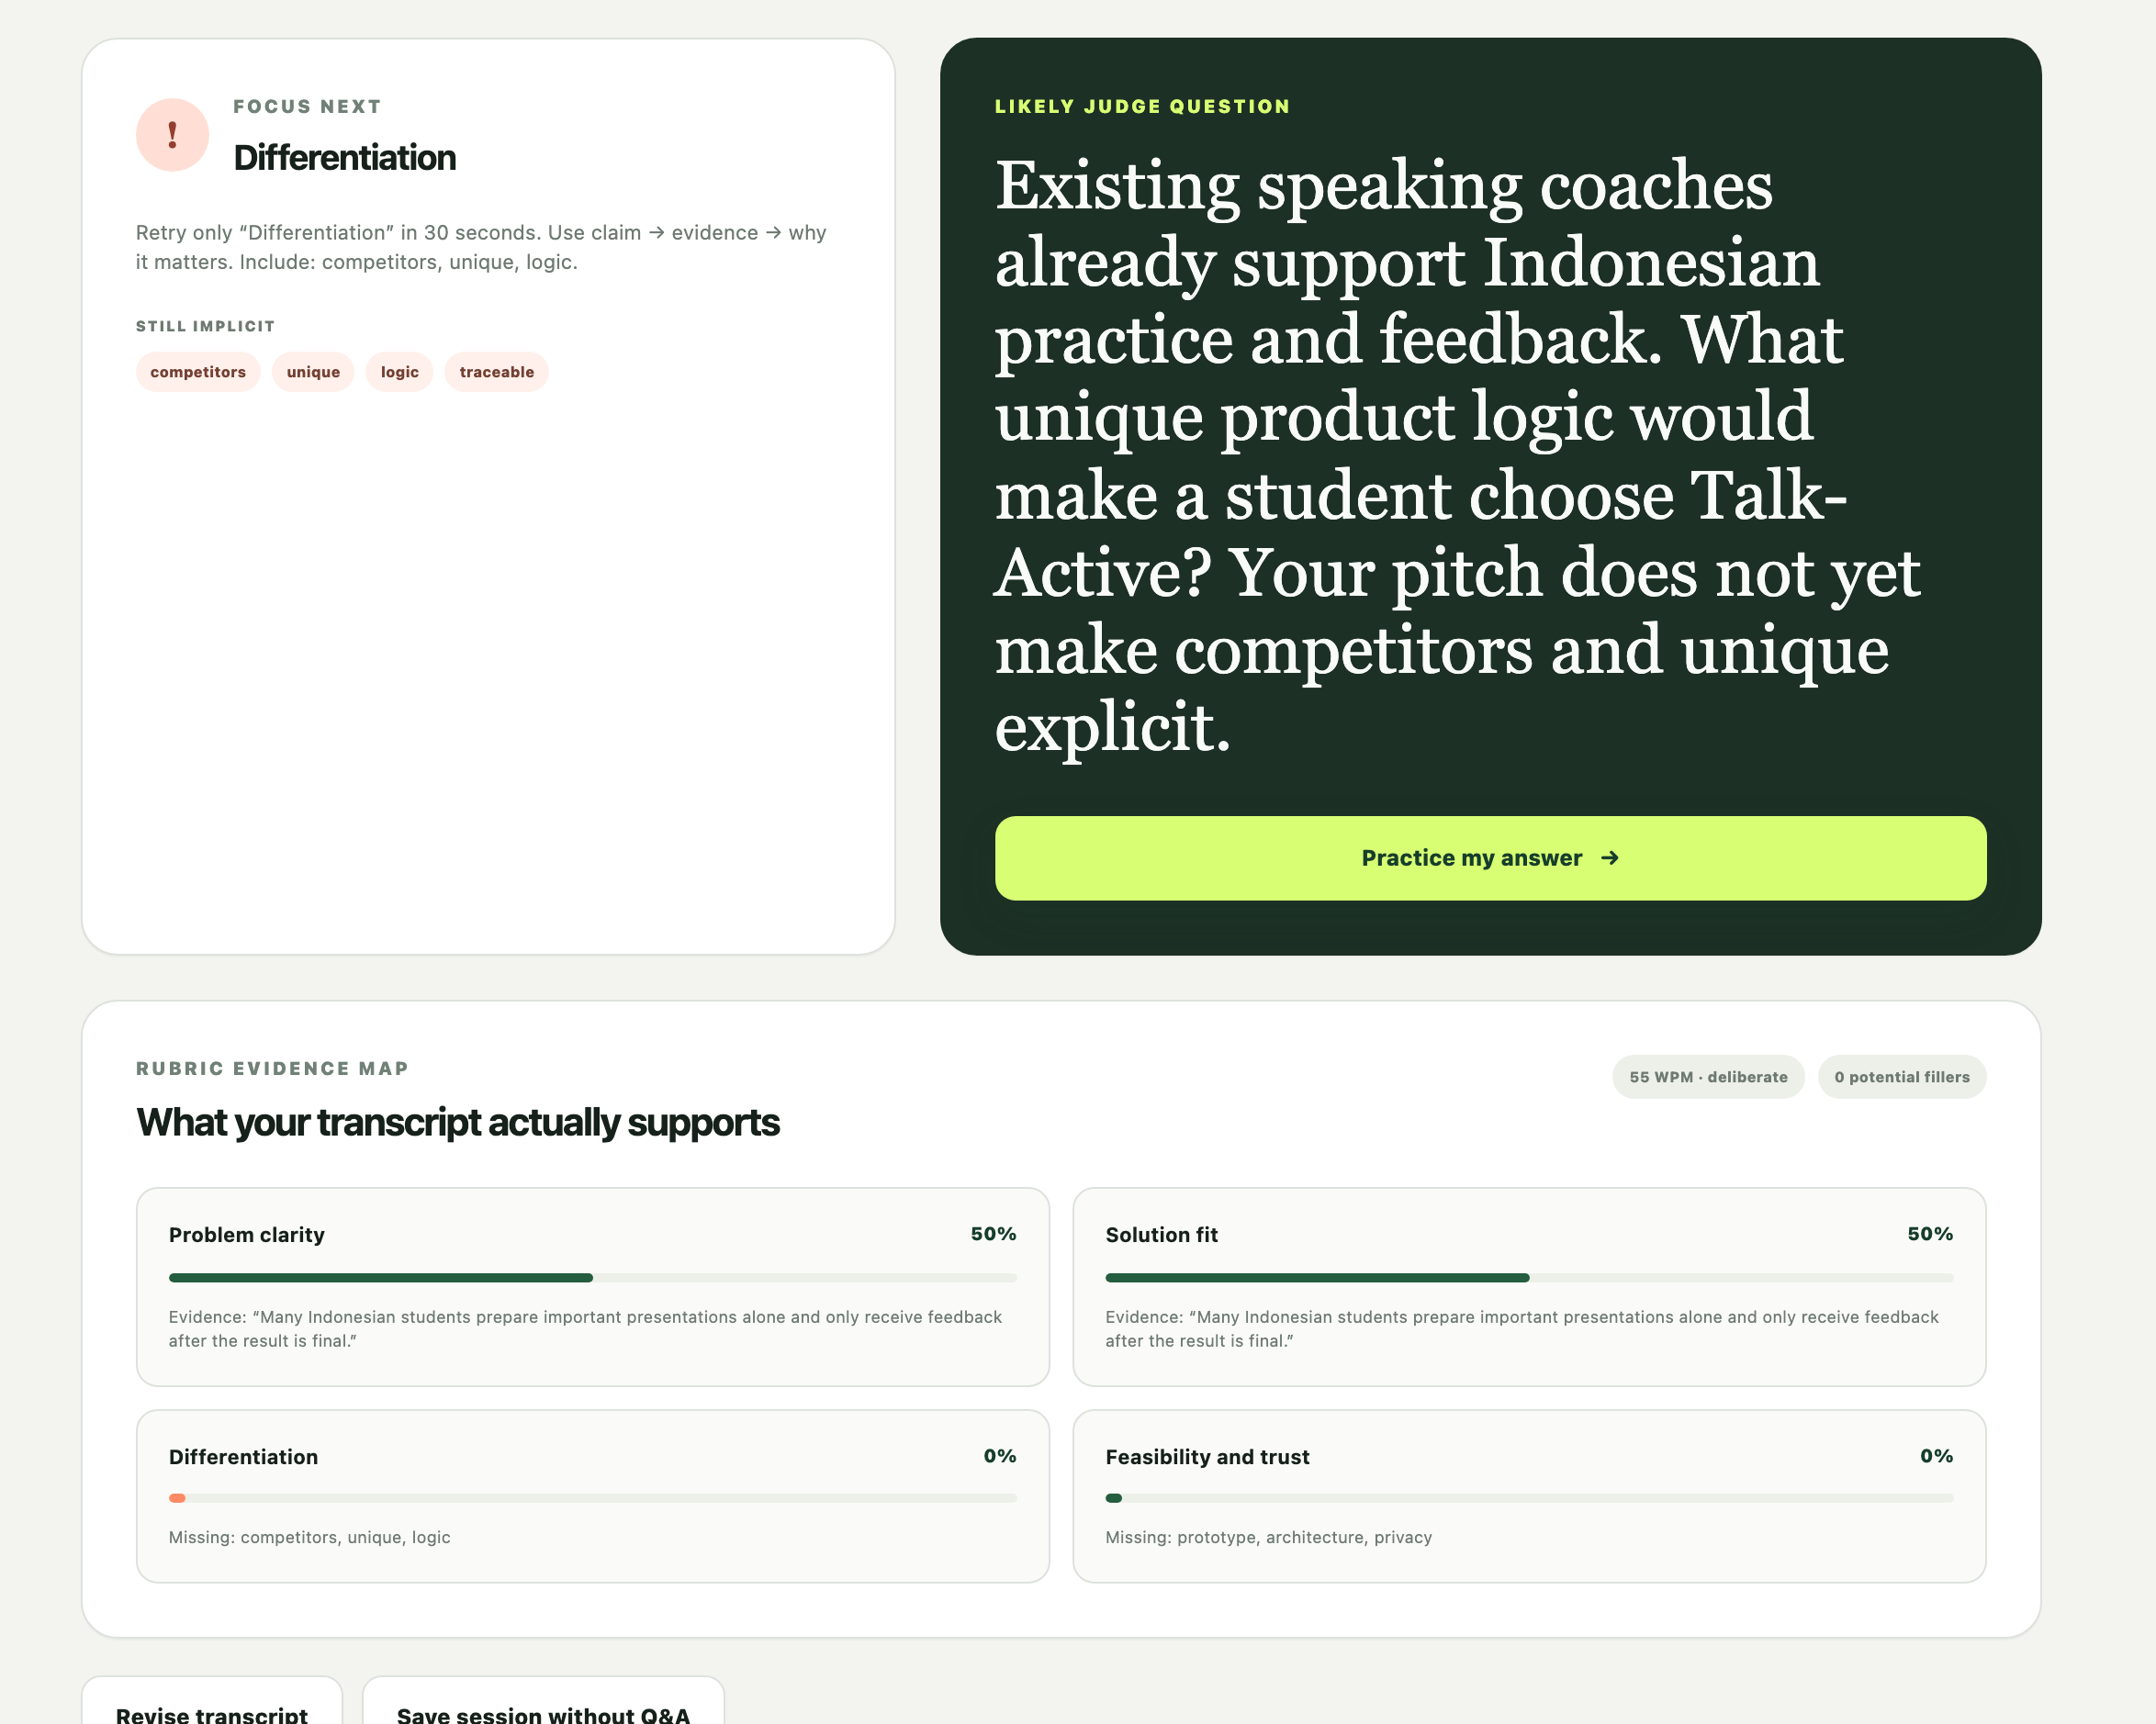
\includegraphics[width=0.66\textwidth]{assets/screens/crop-evidence.png}};

% normalised overlay coordinate system across the image node
\begin{scope}[
  x={($(shot.south east)-(shot.south west)$)},
  y={($(shot.north west)-(shot.south west)$)},
  shift={(shot.south west)}
]
  \node[pin] at (0.048,0.905) {1};
  \node[pin] at (0.048,0.775) {2};
  \node[pin] at (0.505,0.905) {3};
  \node[pin] at (0.048,0.395) {4};
  \node[pin] at (0.048,0.118) {5};
\end{scope}

\draw[rulegrey, line width=0.5pt] (shot.south west) rectangle (shot.north east);

\end{tikzpicture}

\caption{The rubric evidence review, captured from the running prototype.
\textbf{(1)}~the weakest criterion is named, not a vague weakness;
\textbf{(2)}~the evidence still missing is listed as cues to make explicit;
\textbf{(3)}~the judge question is generated from that criterion;
\textbf{(4)}~every criterion cites the exact transcript sentence behind its
verdict; \textbf{(5)}~unsupported criteria name precisely what was absent. This
screen is why \ProductName{} is not a speaking coach: every statement it makes
is anchored to a criterion the evaluator wrote and a sentence the student said.}
\label{fig:mockup}
\end{figure}


A first session runs about twelve minutes: three to set up the project and
rubric, four to deliver the attempt, three to read the evidence map, and two to
answer the judge question. A returning student skips setup and lands straight on
their recurring weakness, which is the behaviour we want the workspace to
produce.

% ----------------------------------------------------------------------------
\section{Business Strategy \& Viability}
% ----------------------------------------------------------------------------

\subsection{Market segments and sizing}

The total market is every student who faces a rubric-scored oral evaluation;
the serviceable market is those in an active evaluation cycle in a given year;
we start somewhere small on purpose, because competition and scholarship
communities already gather in organised groups, already hold a written rubric,
and can be reached without paid acquisition.

% ---------------------------------------------------------------- Figure ----
% TAM / SAM / SOM, built upward from official enrolment data.
\begin{figure}[htbp]
\centering
\begin{tikzpicture}[font=\fontsize{8}{9.5}\selectfont]

\fill[uinavy!22, rounded corners=2pt]      (0,0)      rectangle (13.6,0.86);
\fill[uinavy!48, rounded corners=2pt]      (2.15,0.97) rectangle (11.45,1.83);
\fill[ristekpurple!85, rounded corners=2pt] (4.75,1.94) rectangle (8.85,2.80);

\node[text=inkgrey, font=\fontsize{8.4}{10}\selectfont\bfseries] at (6.8,0.60)
  {TAM \textperiodcentered{} 9.95 million};
\node[text=inkgrey!85, font=\fontsize{7.4}{9}\selectfont] at (6.8,0.26)
  {all Indonesian higher-education students \cite{pddikti2025}};

\node[text=white, font=\fontsize{8.4}{10}\selectfont\bfseries] at (6.8,1.57)
  {SAM \textperiodcentered{} about 2.0 million per year};
\node[text=white, font=\fontsize{7.4}{9}\selectfont] at (6.8,1.23)
  {final-year defenders, competition entrants, scholarship and graduate applicants};

\node[text=white, font=\fontsize{8.4}{10}\selectfont\bfseries] at (6.8,2.54)
  {SOM \textperiodcentered{} about 60,000};
\node[text=white, font=\fontsize{7.4}{9}\selectfont] at (6.8,2.20)
  {UI and peer-university competition \& scholarship communities, years 1--3};

\end{tikzpicture}
\caption{Market sizing built upward from official enrolment data, narrowing to a
beachhead reachable through the student-organisation channels we already belong
to.}
\label{fig:market}
\end{figure}


\subsection{Revenue model}

\begin{table}[htbp]
\centering
\caption{Revenue model: free core loop, paid depth, institutional scale.}
\label{tab:revenue}
{\fontsize{10.5}{13}\selectfont
\begin{tabularx}{\textwidth}{@{}L{2.5cm} L{3.5cm} X@{}}
\toprule
\textbf{Tier} & \textbf{Price} & \textbf{Includes} \\
\midrule
\textbf{Free} & Rp0 &
One active project, three analysed sessions per month. The full loop is
never paywalled, because equity is the point of the product. \\
\addlinespace
\textbf{Pro} & Rp39,000/month &
Unlimited projects and sessions, document import, recording and
transcription, deeper evidence analysis, and export. \\
\addlinespace
\textbf{Campus} & Rp25--50 million/year per faculty &
Site licence for a faculty or study programme, cohort-level recurring-weakness
analytics for lecturers, and thesis-defense rubric templates. \\
\addlinespace
\textbf{Partner} & Sponsored &
Scholarship providers and graduate recruiters sponsoring preparation tracks
for their own published criteria. \\
\bottomrule
\end{tabularx}}
\end{table}

Unit economics are governed by model inference. A full analysed session costs
an estimated Rp900--1,800, so a Pro subscriber carries a gross margin above
70\%, and the free tier's three-session cap bounds subsidy to roughly Rp5,400
per user per month. Caching rubric parses and reserving the largest model for
evidence mapping are the levers that control this cost.

\textbf{Go-to-market.} We start where we already stand: UI student
organisations, competition communities, and the Fasilkom UI thesis cohort.
Distribution runs through the same channels students already use to find
rubrics. Institutional conversations follow evidence of student outcomes, not
before it. The Campus tier is sold on cohort data the free tier generates.

% ----------------------------------------------------------------------------
\section{Expected Results}
% ----------------------------------------------------------------------------

\subsection{Target metrics}

\begin{table}[htbp]
\centering
\caption{Quantifiable targets. Product metrics are primary; delivery metrics
are supporting context only.}
\label{tab:metrics}
{\fontsize{10.5}{13}\selectfont
\begin{tabularx}{\textwidth}{@{}X L{3.0cm} L{2.6cm}@{}}
\toprule
\textbf{Metric} & \textbf{Target} & \textbf{Horizon} \\
\midrule
Students who return for a second session (core validity signal) &
≥40\% & 3 months \\
Rubric-criterion coverage improvement between attempt 1 and attempt 3 &
≥25 percentage points & Per user \\
Students who revise a specific claim after the evidence review &
≥60\% & 3 months \\
Rubric import parsed correctly without manual correction &
≥85\% & 6 months \\
Registered students / paying conversion & 10,000 / 5\% & 12 months \\
Faculty site licences & 3 & 12 months \\
\bottomrule
\end{tabularx}}
\end{table}

The first metric is the one that matters. A student who does not come back has
not been helped, whatever the interface looked like.

\subsection{User benefits}

\begin{itemize}
  \item \textbf{Equitable access.} Rigorous, rubric-grounded rehearsal without
        needing a mentor, an alumni network, or the money for a coach.
  \item \textbf{Actionable rather than generic feedback.} ``Criterion 3 asks
        for field data; your pitch offered an anecdote'' is something a student
        can fix tonight. ``Be more confident'' is not.
  \item \textbf{Rehearsed under pressure.} The interrogation is practised, not
        just the presentation, which is the part students consistently skip.
  \item \textbf{Cumulative and low risk.} Progress is retained across sessions,
        so a student can see whether a weakness is closing, and nothing is kept
        beyond the transcript they control.
\end{itemize}

% ----------------------------------------------------------------------------
\section{Scalability \& Future Roadmap}
% ----------------------------------------------------------------------------

% ---------------------------------------------------------------- Figure ----
% Scaling roadmap as a compact single-row strip of five cards.
\begin{figure}[htbp]
\centering
\begin{tikzpicture}[font=\fontsize{7.4}{8.8}\selectfont]

% Explicit dimensions: five 2.72 cm cards with 0.28 cm gutters spans 14.72 cm,
% which fits inside the 15 cm text block.
\newcommand{\CardW}{2.72}   % card width in cm (unitless for coordinates)
\newcommand{\Pitch}{3.00}   % card width + gutter

% #1 index (0-based)  #2 accent colour  #3 title  #4 when  #5 body
\newcommand{\phase}[5]{%
  \pgfmathsetmacro{\X}{#1*\Pitch}%
  \node[anchor=north west,
        draw=#2!45, fill=#2!7, line width=0.55pt, rounded corners=2.5pt,
        inner sep=4pt,
        text width=2.34cm,          % 2.72cm card - 2*4pt inner sep
        align=flush left,
        minimum width=2.72cm, minimum height=2.30cm]
    at (\X,0)
    {{\fontsize{8}{9.4}\selectfont\bfseries\color{inkgrey}#3}\\[1.5pt]
     {\fontsize{6.9}{8.2}\selectfont\itshape\color{#2}#4}\\[3pt]
     {\fontsize{6.9}{8.3}\selectfont\color{inkgrey!88}#5}};
}

\phase{0}{goodgreen}{Prototype}{shipped}%
  {Full loop, persistence, and a passing automated gate.}
\phase{1}{ristekpurple}{Innovation Week}{10--14 Aug 2026}%
  {Semantic evidence mapping with cited spans; rubric import.}
\phase{2}{uinavy}{Validation}{Year 1}%
  {Accounts, consent, deletion. Ten-student study.}
\phase{3}{uinavy}{Adjacent contexts}{Year 2}%
  {Thesis defense, LPDP panels, job interviews.}
\phase{4}{uired}{Institutional}{Year 3}%
  {Campus licences and cohort analytics for lecturers.}

% progression arrows sitting in the gutters
\foreach \i in {0,1,2,3}{
  \pgfmathsetmacro{\AX}{\i*\Pitch+\CardW}
  \draw[-{Stealth[length=3.2pt]}, draw=inkgrey!50, line width=0.6pt]
    (\AX,-1.15) -- ({\AX+0.26},-1.15);
}

\end{tikzpicture}
\caption{Scaling roadmap. What compounds is the library of parsed Indonesian
rubric archetypes, not the infrastructure.}
\label{fig:roadmap}
\end{figure}


Scaling is a matter of \textbf{rubric coverage}, not infrastructure: the
serverless stack already scales with demand and to zero when idle. What
compounds is the library of parsed rubric archetypes. Every thesis form,
scholarship guide, and competition matrix the system learns to structure makes
the next student's setup faster. Because rubrics are institution-specific, a
global competitor cannot replicate that library from outside Indonesia.

\textbf{Post-hackathon path.} Straight after Innovation Week we run the
validation study with the Fasilkom UI thesis cohort, then extend to two further
faculties. UI Incubate is the intended vehicle for turning the first Campus
licences into a sustainable operation.

\textbf{Validation before scale.} We will give ten students their own rubric
and observe two sessions each. Success is not a satisfaction score but whether a
student \emph{changes a specific claim} because the review exposed it.
Appendix~A sets out the principal risks.
